\documentclass[12pt, a4paper]{article}

\usepackage[T1]{fontenc}
\usepackage[utf8]{inputenc}
\usepackage[portuguese]{babel}
\usepackage{indentfirst}
\usepackage[table,xcdraw]{xcolor}
\usepackage{graphicx}

\usepackage{geometry}
\geometry{a4paper, margin=25mm}

\graphicspath{{./Figures/}}

\usepackage[
    backend=biber,
    sorting=none]{biblatex}
\addbibresource{ref.bib}



\title{Assignment 1}
\author{Hélder Vieira\\Miguel Tavares}
\date{14 de Abril de 2021}



\begin{document}



\maketitle


\section{Introdução} % (fold)
\label{sec:introdução}

No mundo actual existem cada vez mais dados disponíveis sobre o dia a
dia de um cidadão normal, quer seja através da utilização dos mais
diversos dispositivos como através da utilização de serviços colectivos
em grandes centros urbanos. De forma a tirar partido desta enorme
quantidade de dados para chegar a conclusões viáveis em tempo útil, é
necessário fazer uso dos métodos disponíveis para redução de variáveis e
explicação de variância. Com isto é possível aumentar o rendimento das
análises dos dados. Neste projecto foi
proposto a escolha de um \emph{dataset} com determinadas características
e a realização de diversos tipos de análises, univariada, bivariada e
multivariada, aos dados obtidos. Numa
primeira parte será exposto uma breve análise dos dados agrupados por
continentes, de forma a dar uma visão mais geral ao leitor, e também de
contextualizar com a realidade actual. De seguida, cada variável será
analisada com o intuito de se perceber como estão distribuídas.
Posteriormente, o alvo de estudo será a relação entre essas mesmas
variáveis e a sua influência, principalmente no \emph{Score} de cada
país. Na segunda e última parte serão
abordados os métodos de \emph{Factor Analysis} de forma a avaliar o peso
de cada variável nas restantes. Os dados serão normalizados de forma a
que os consigamos analisar na mesma escala de grandeza e avaliados sobre
a sua adequação. Para terminar, uma \emph{Principal Component Analysis}
será realizada e conclusões de como algumas variáveis são mais
relevantes do que outras.

% section introdução (end)


\section{Análise de Dados} % (fold)
\label{sec:análise_de_dados}

\subsection{Introdução} % (fold)
\label{sub:introdução}


Para a realização deste trabalho foi escolhido um dataset que traduz o
nível de felicidade, bem como outros indicadores, de diversos países,
relativo ao ano de 2019. Uma vez que cada entrada correspondia a um
país, decidiu-se agrupar os dados pelo continente ao qual os países
pertencem. Começando pelo \emph{Score}, este
é baseado nas respostas de um questionário sobre a avaliação da
qualidade de vida da população. Na questão, conhecida como \emph{Escada
de Cantril} é pedido que se imagine uma escada com 10 degraus (0 em
baixo e 10 no topo). O décimo degrau corresponde à melhor vida que o
questionado poderia ter, e o primeiro, a pior \cite{kaggle}.

\begin{figure}[h]
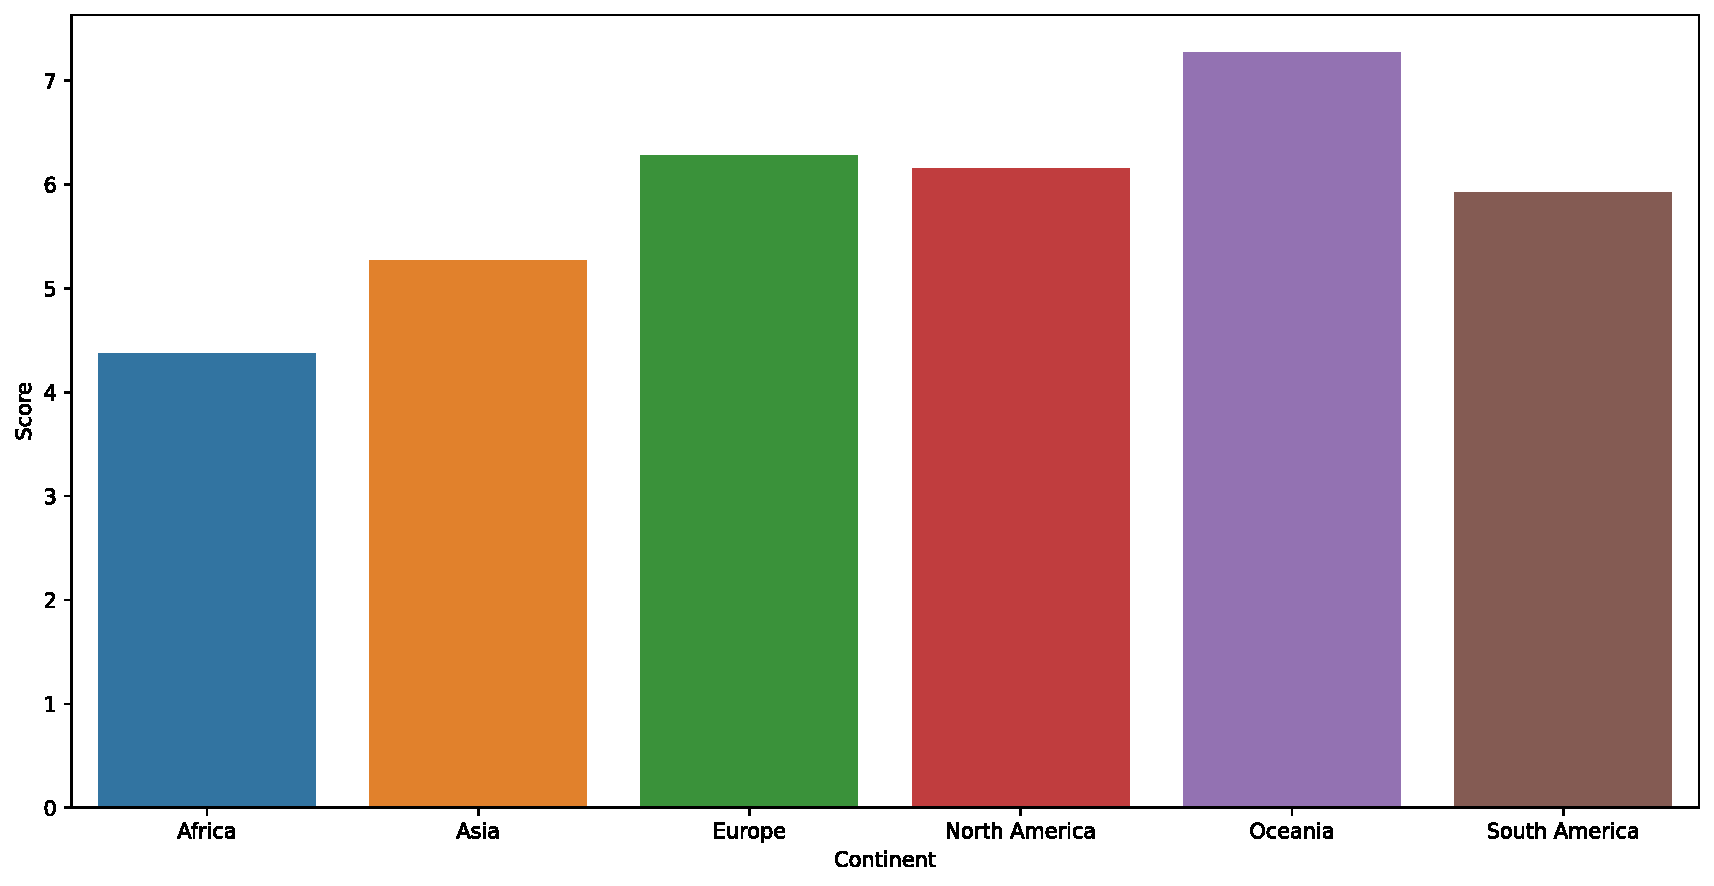
\includegraphics[scale=0.45]{score_continents.pdf}
\centering
\caption{\emph{Média de Score por Continente}}
\label{fig:fig1}
\end{figure}

Na Figura~\ref{fig:fig1} podemos observar a média dos \emph{Scores} dos diversos
países pelo continente ao qual pertencem. Rapidamente se observa que
continentes onde se encontram os países mais desenvolvidos são os que,
em média, têm um \emph{Score} mais elevado. Na Figura~\ref{fig:fig2} abaixo podemos
observar a distribuição do \emph{Score} pelos diversos países do mundo.

\begin{figure}[h]
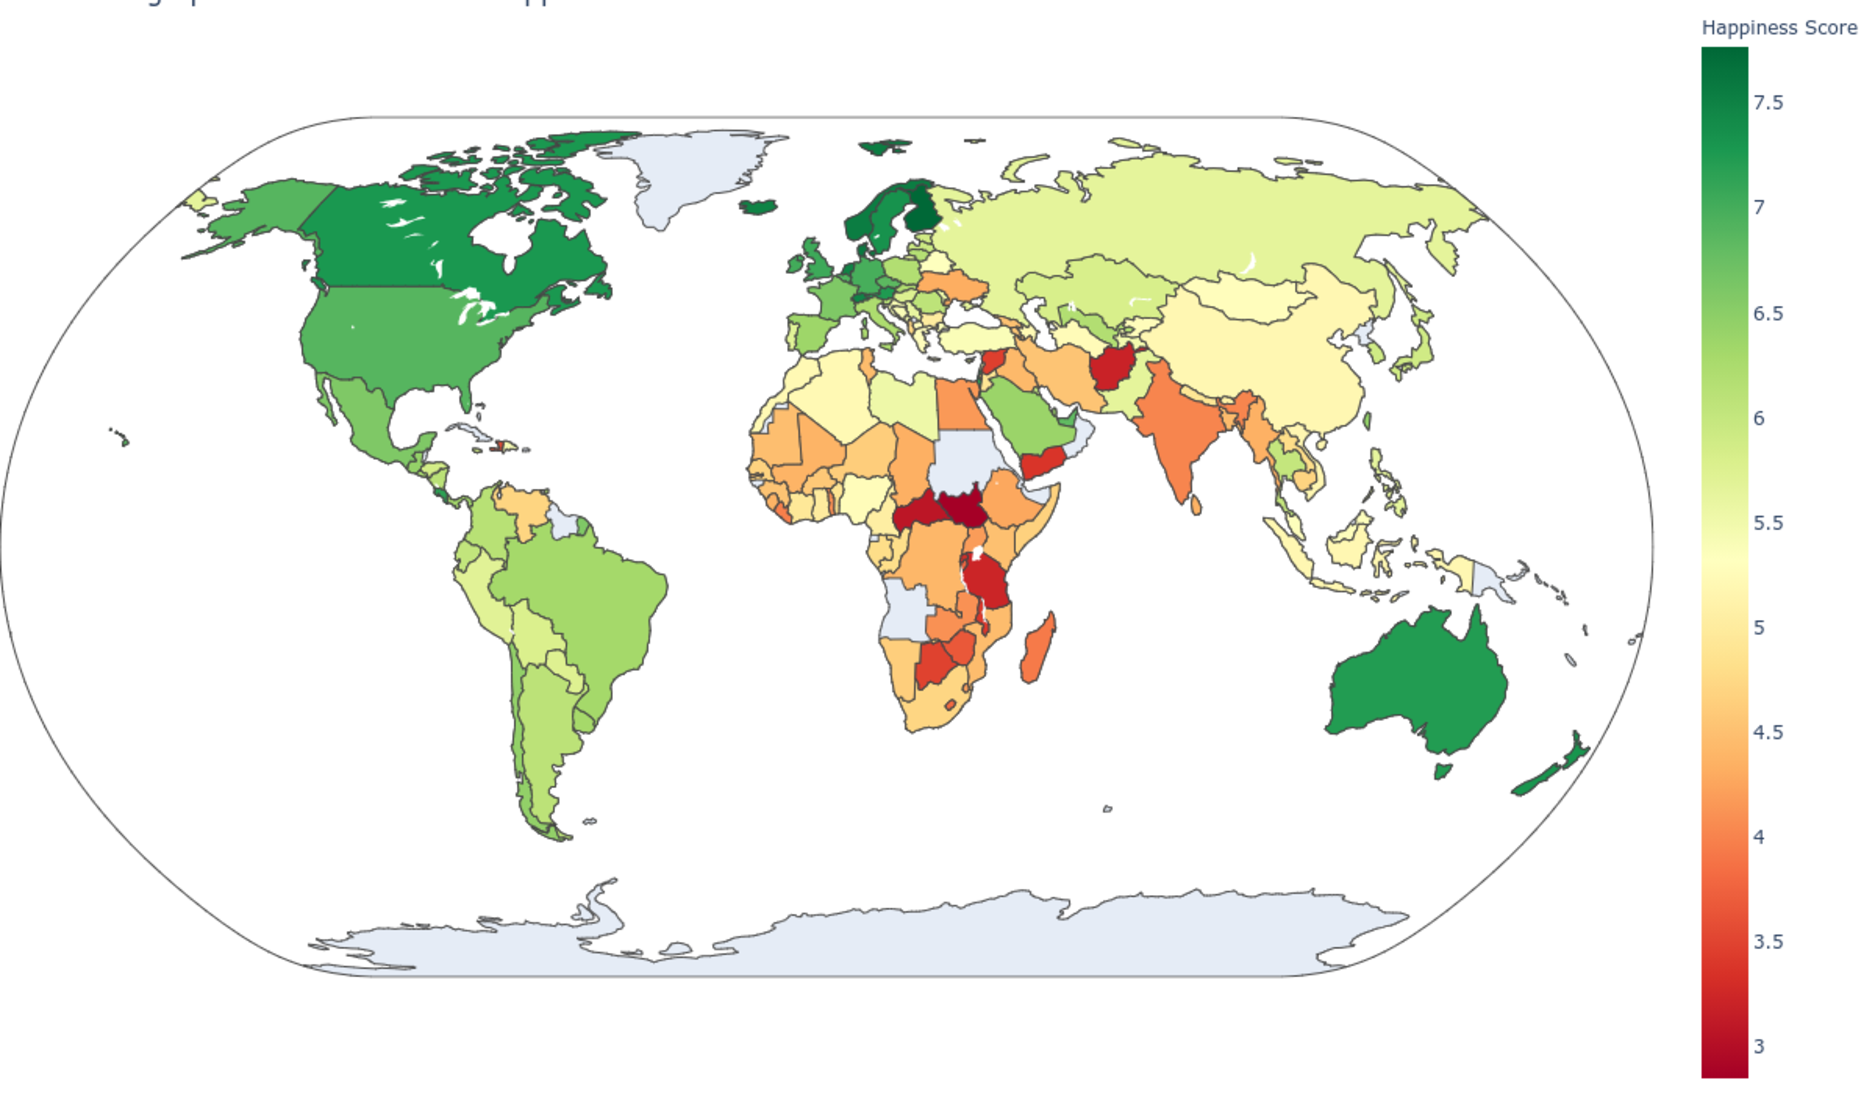
\includegraphics[scale=0.40]{score-worldmap.pdf}
\centering
\caption{\emph{Score dos diversos países}}
\label{fig:fig2}
\end{figure}

Existem outros factores que estão fortemente relacionados, mas sem
impacto, com o \emph{Score}, tais como o \emph{GDP per capita (PIB per
capita), Social support (apoios sociais), Healthy life expectancy
(esperança média de vida), Freedom to make life choices (liberdade),
Generosity (generosidade) e Perception of corruption (Corrupção)}. É
importante realçar que todos estes factores são também resultados de
questionários, expecto o PIB per capita e a esperança média de
vida. Uma nota para a variável
\emph{Corrupção}. Esta não representa o quão corrupto é um país, mas sim
a capacidade da população em detectar/identificar corrupção.

\begin{figure}[h]
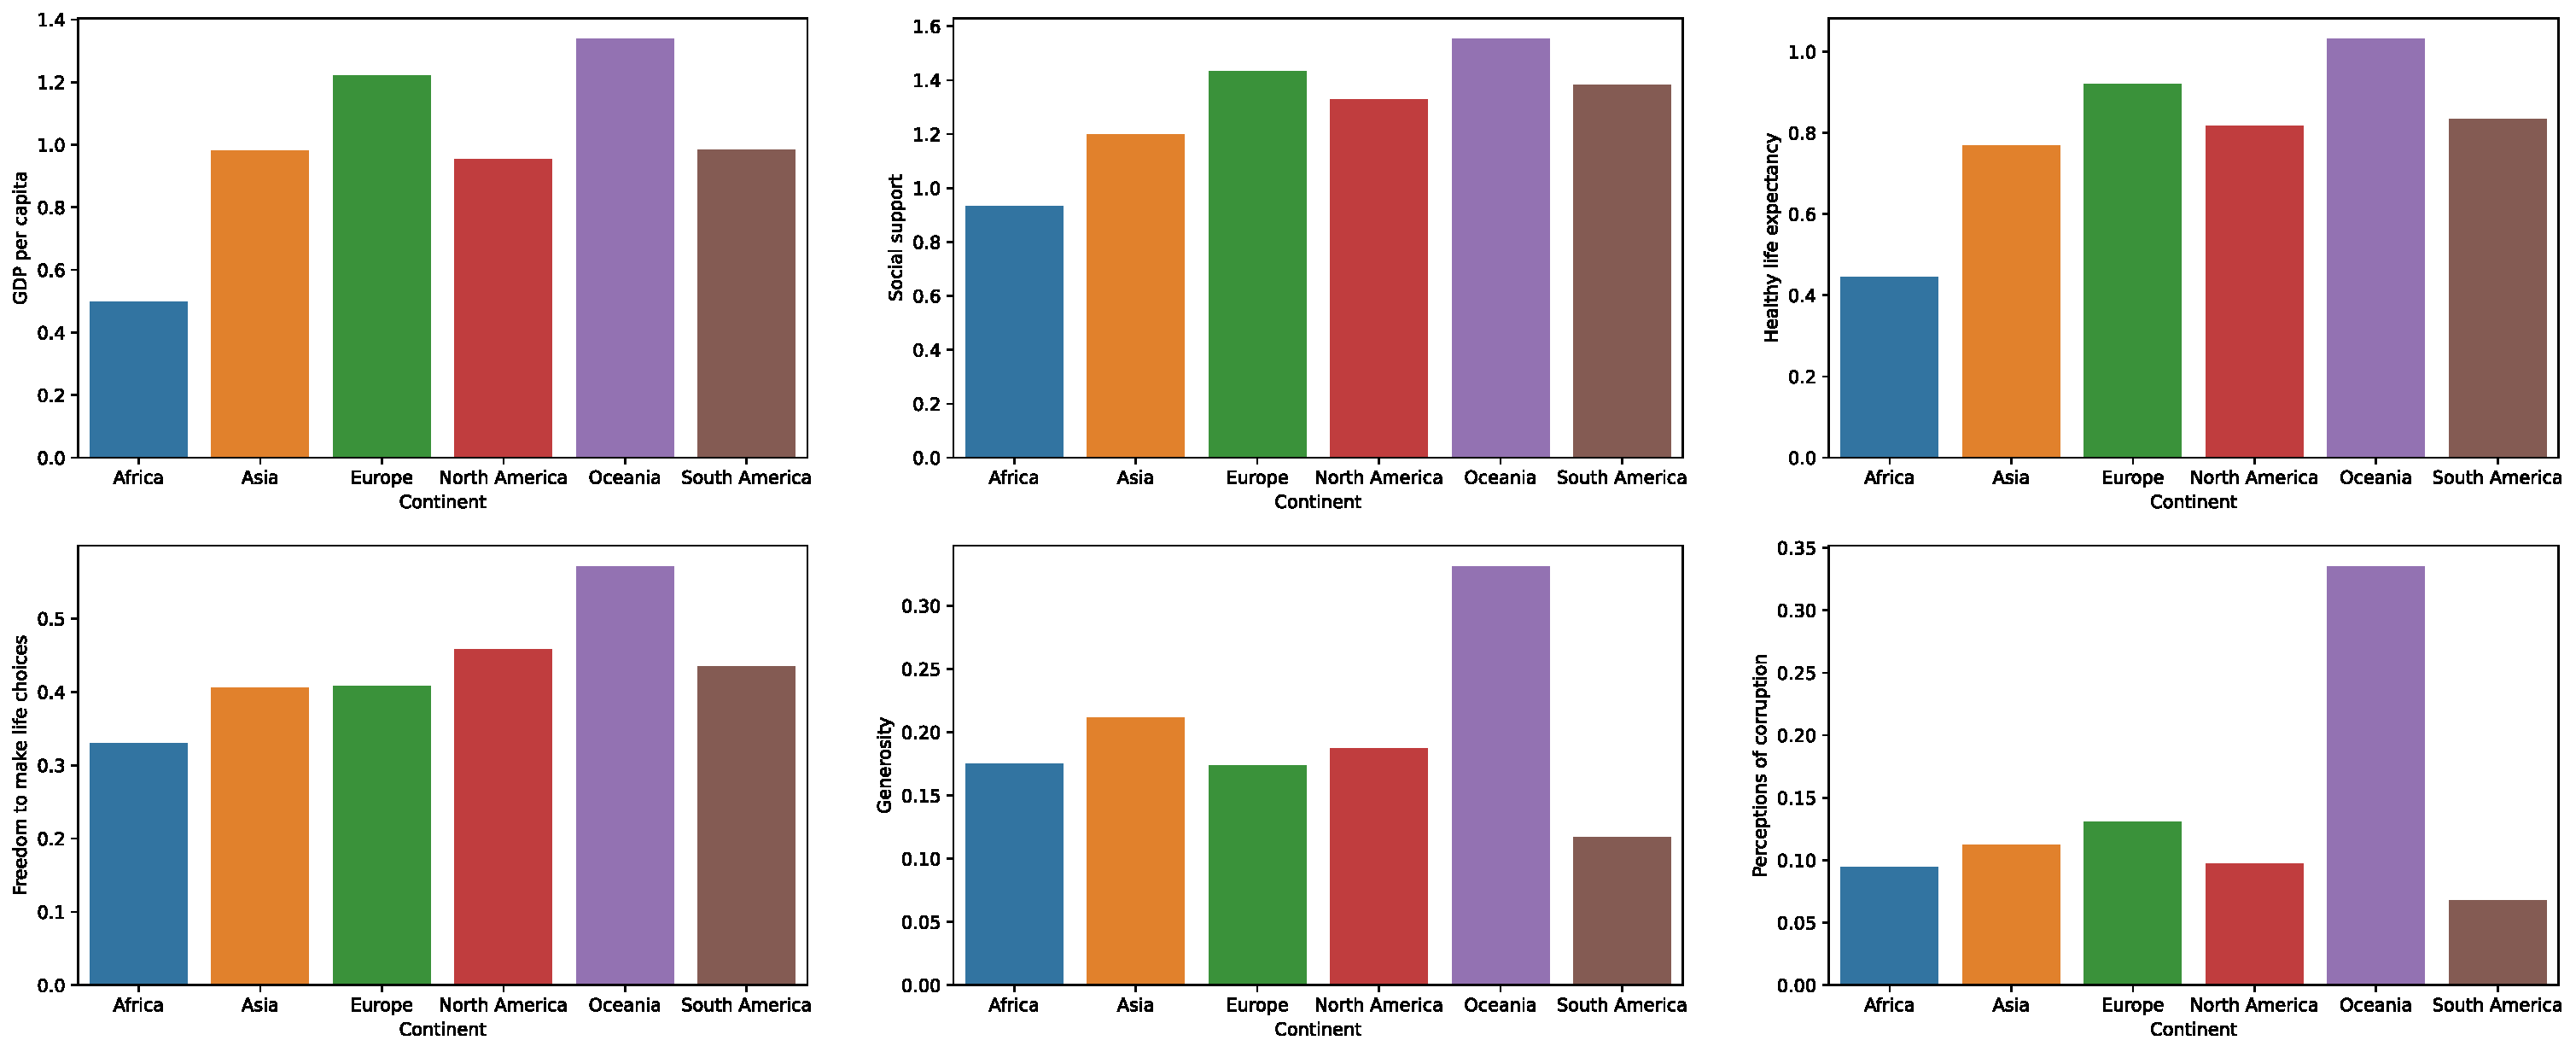
\includegraphics[scale=0.30]{variables-continents.pdf}
\centering
\caption{\emph{Média dos restantes factores por continente}}
\label{fig:fig3}
\end{figure}

Como observável na Figura~\ref{fig:fig3}, todos os indicadores seguem o \emph{Score}. Relativamente
à generosidade e corrupção, a Oceania apresenta valores de média muito
mais elevados que os restantes continentes devido ao facto de a sua
amostra é constituída por apenas dois países de elevado índice de
desenvolvimento. Para concluir, através de
uma análise rápida dos dados agrupados por continente, fica retida a
ideia que os países considerados desenvolvidos vão obter resultados mais
elevados, e que esses mesmo países se encontram, na sua maioria, no
hemisfério norte.


% subsection introdução (end)


\subsection{Análise Univariada} % (fold)
\label{sub:análise_univariada}


Neste capítulo será realizada uma análise estatística a cada uma das
variáveis presentes no \emph{dataset}. Analisando a Tabela~\ref{tab:tab1} abaixo
representada podemos retirar algumas conclusões:

\begin{itemize}
\item
  O número de países representados é de 156;
\item
  A média do \emph{Score} está próximo do meio da escala e o valor
  máximo é de 7.77 e mínimo de 2.85;
\item
  Metade dos países representados têm um \emph{Score} compreendido entre
  4.5 e 6.2;
\item
  Alguns países não têm dados relativos aos factores em causa, pois
  temos mínimos de 0;
\item
  As respectivas médias e medianas andam próximas, de onde concluímos
  que a distribuição dos valores será aproximadamente centrada.
\end{itemize}

\begin{table}[ht]
\centering
\begin{tabular}{|l|c|c|c|c|c|c|c|}
\hline
\textit{\textbf{}} & \textit{\textbf{Score}} & \textit{\textbf{\begin{tabular}[c]{@{}c@{}}GDP\\ per\\ Capita\end{tabular}}} & \textit{\textbf{\begin{tabular}[c]{@{}c@{}}Social\\ support\end{tabular}}} & \textit{\textbf{\begin{tabular}[c]{@{}c@{}}Healthy\\ life\\ expectancy\end{tabular}}} & \textit{\textbf{\begin{tabular}[c]{@{}c@{}}Freedom\\ to make\\ life\\ choices\end{tabular}}} & \textit{\textbf{Generosity}} & \textit{\textbf{\begin{tabular}[c]{@{}c@{}}Perceptions\\ of\\ corruption\end{tabular}}} \\ \hline
count & 156 & 156 & 156 & 156 & 156 & 156 & 156 \\ \hline
mean & 5.407 & 0.905 & 1.208 & 0.725 & 0.392 & 0.184 & 0.110 \\ \hline
std & 1.113 & 0.398 & 0.299 & 0.242 & 0.143 & 0.095 & 0.094 \\ \hline
min & 2.853 & 0.000 & 0.000 & 0.000 & 0.000 & 0.000 & 0.000 \\ \hline
25\% & 4.544 & 0.602 & 1.055 & 0.547 & 0.308 & 0.108 & 0.047 \\ \hline
50\% & 5.379 & 0.960 & 1.271 & 0.789 & 0.417 & 0.177 & 0.085 \\ \hline
75\% & 6.184 & 1.232 & 1.452 & 0.881 & 0.507 & 0.248 & 0.141 \\ \hline
max & 7.769 & 1.684 & 1.624 & 1.141 & 0.631 & 0.566 & 0.453 \\ \hline
IQR & 1.640 & 0.629 & 0.396 & 0.334 & 0.199 & 0.139 & 0.094 \\ \hline
skew & 0.011 & -0.385 & -1.134 & -0.613 & -0.685 & 0.745 & 1.650 \\ \hline
mad & 0.916 & 0.332 & 0.236 & 0.199 & 0.116 & 0.075 & 0.069 \\ \hline
kurt & -0.608 & -0.769 & 1.229 & -0.302 & -0.068 & 1.173 & 2.416 \\ \hline
\end{tabular}
\caption{\emph{Descrição estatística}}
\label{tab:tab1}
\end{table}

Analisando o valor de \emph{skewness} concluímos que não temos nenhuma
das variáveis totalmente simétricas quanto à sua distribuição. Por
outras palavras, a \emph{skewness} traduz a falta de simetria das
distribuições. Adicionando a análise de \emph{Kurtosis}, podemos
identificar alguns casos em que a presença de \emph{outliers} é bastante
provável (\emph{p.e. Perceptions of corruption}).

\begin{figure}[ht!]
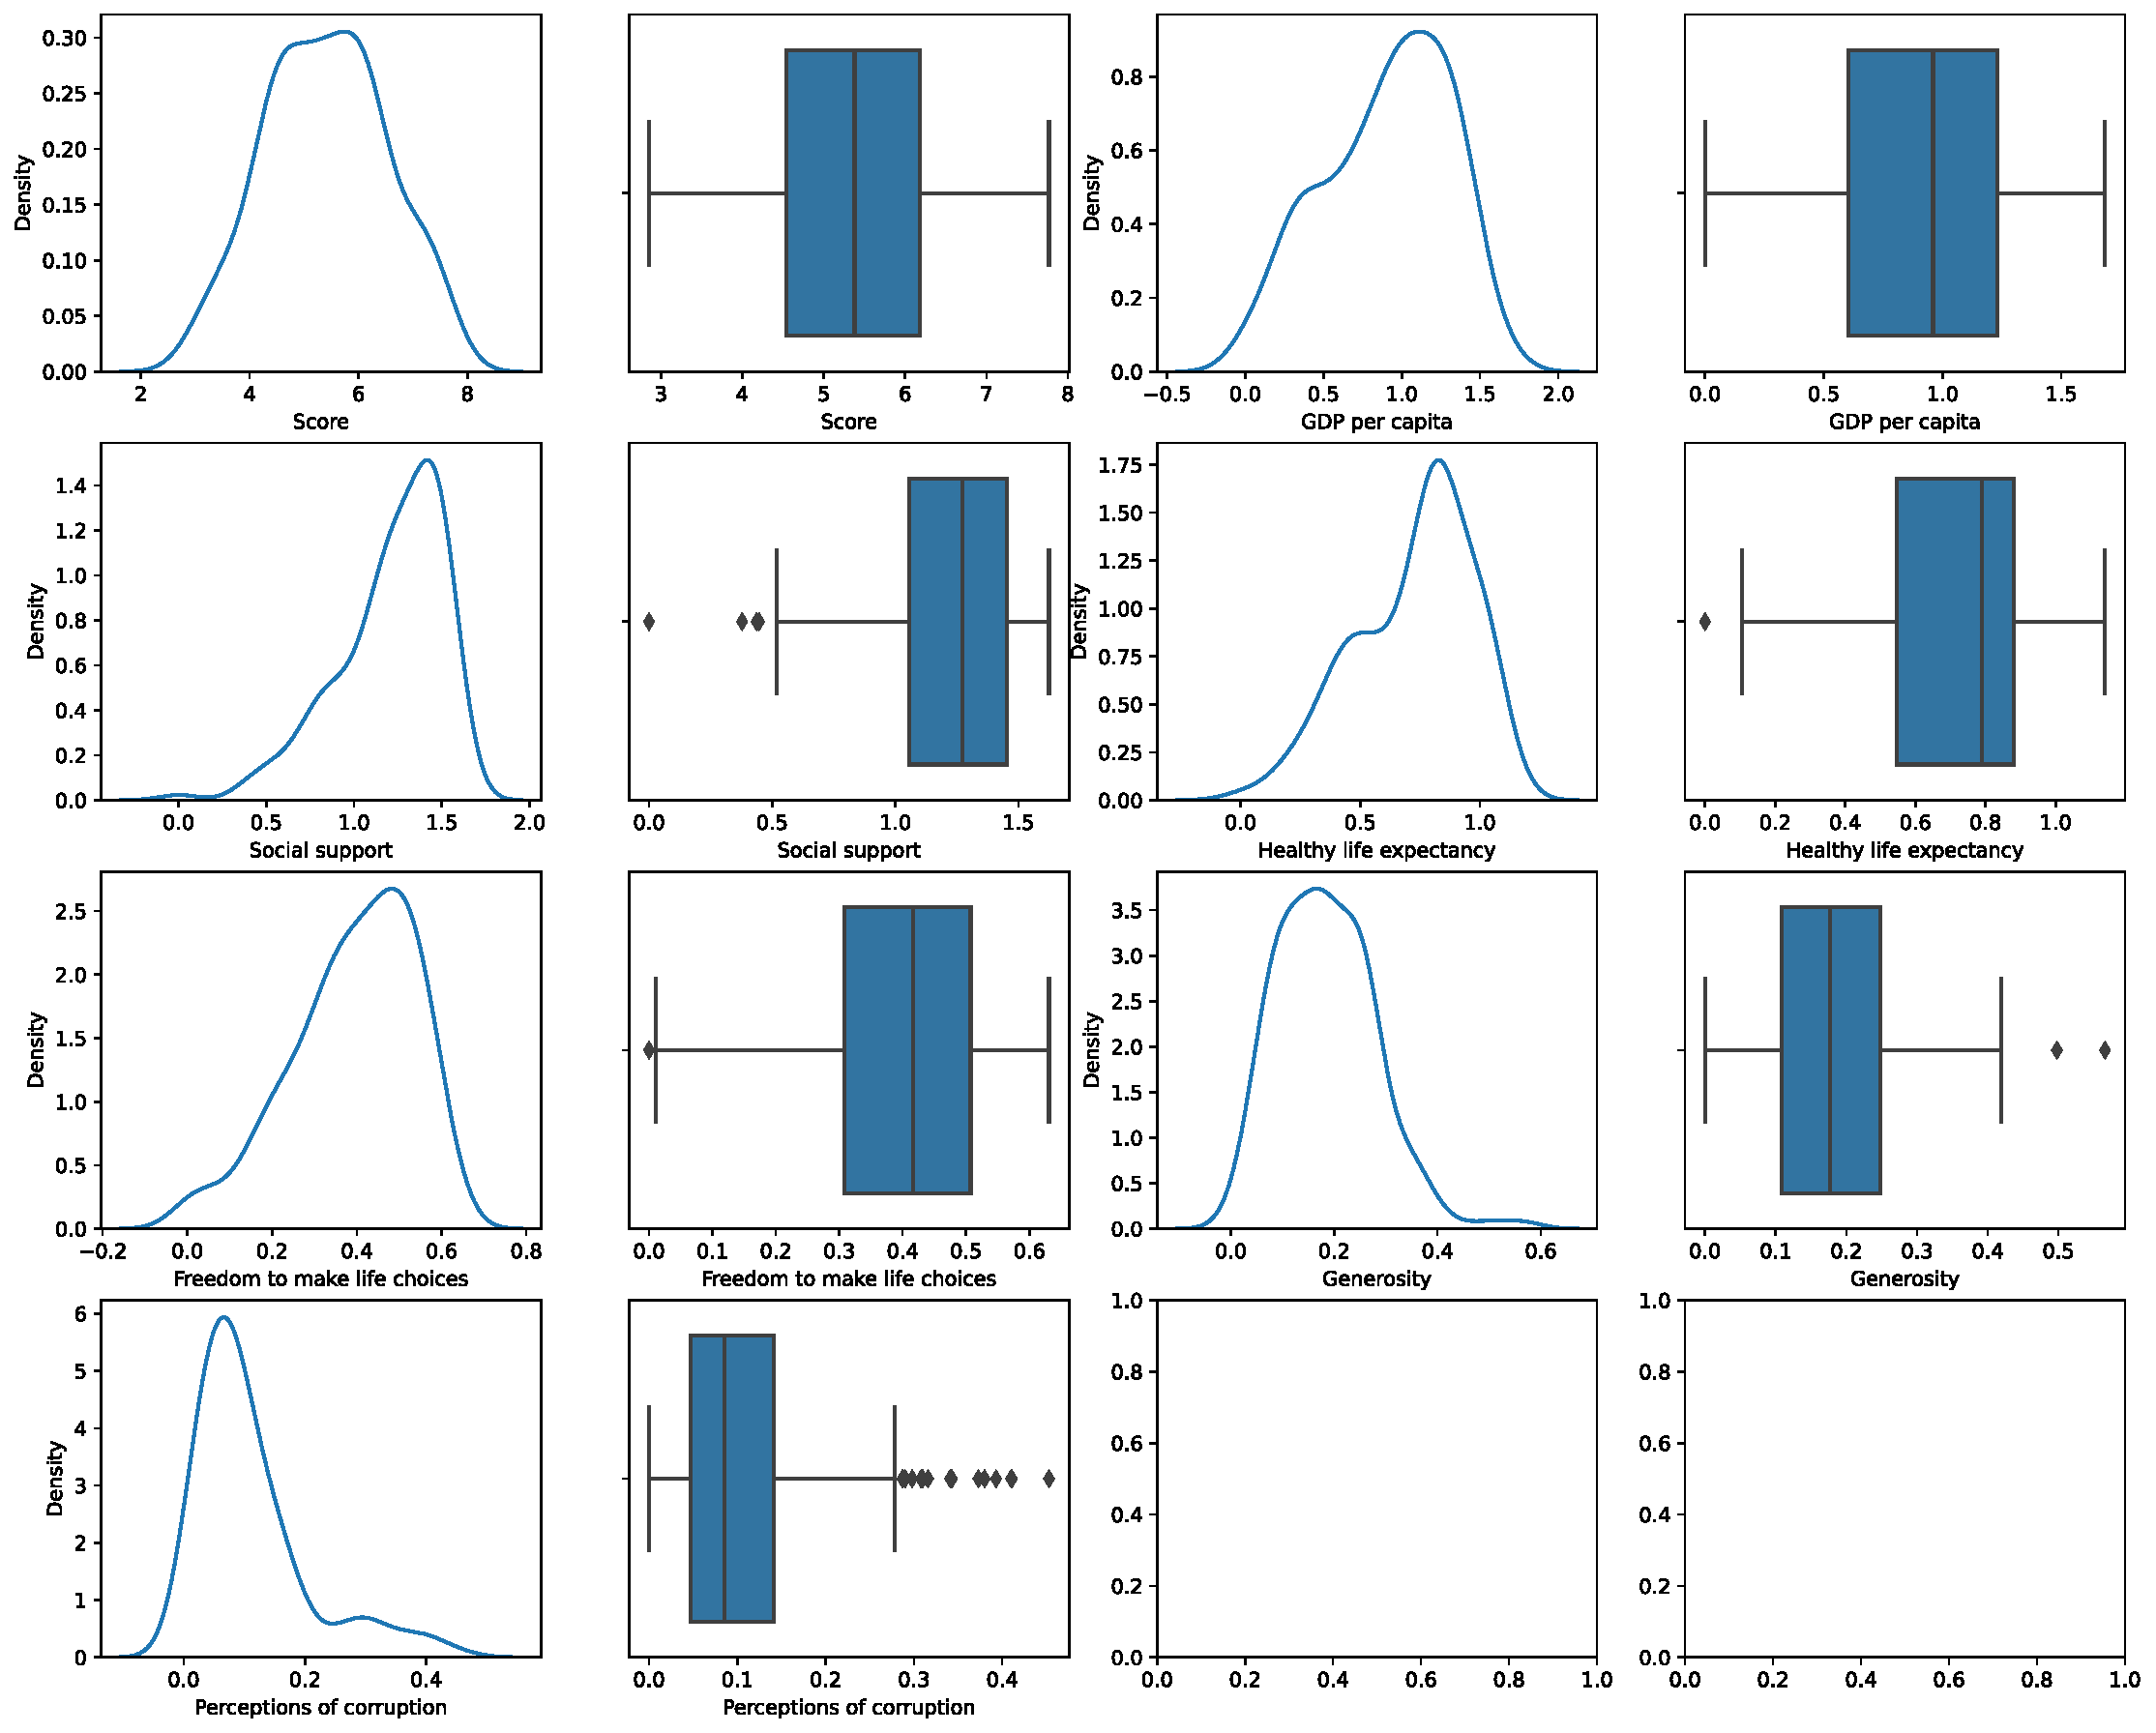
\includegraphics[scale=0.43]{boxplots3.pdf}
\centering
\caption{\emph{Distribuições e boxplots}}
\label{fig:fig4}
\end{figure}

Recorrendo à análise gráfica ilustrada na Figura~\ref{fig:fig4} as conclusões convergem. Todas as distribuições são aproximadamente simétricas, com a presença dos
expectáveis \emph{outliers}. Alguns deles correspondem aos valores em
falta de alguns países. Contudo, a sua existência é única, e por isso,
não significativa. Como esperado, na
corrupção temos a presença de um número maior de \emph{outliers}, o que
vai de encontro ao respectivo valor de
\emph{Kurtosis}. Concluindo, não existe uma
grande disparidade em relação ao \emph{Score} e ao \emph{GDP per capita
(PIB per capita)} dentro dos países analisados. Relativamente ao
\emph{Social support (apoios sociais)} e à \emph{Healthy life expectancy
(esperança média de vida)}, as populações têm uma visão positiva do seu
país. O mesmo pode ser dito da \emph{Freedom to make life choices
(liberdade)}. Por último, \emph{Generosity (generosidade)} e
\emph{Perception of corruption (Corrupção)}, com uma performance menos
boa. A corrupção, como foi dito anteriormente, traduz a percepção de
corrupção. Logo podemos concluir que a presença de \emph{outliers}
corresponde às populações dos países mais desenvolvidos, possivelmente
devido ao maior nível educacional das mesmas.

% subsection análise_univariada (end)


\subsection{Análise Bivariada} % (fold)
\label{sub:análise_bivariada}

Neste capítulo será analisada a relação entre as variáveis. Os casos
mais pertinentes serão quase sempre relativos à relação com o
\emph{Score}. No entanto, a análise de outras relações pode ser útil de
forma a clarificar, indirectamente, alguns tópicos.

\begin{figure}[h]
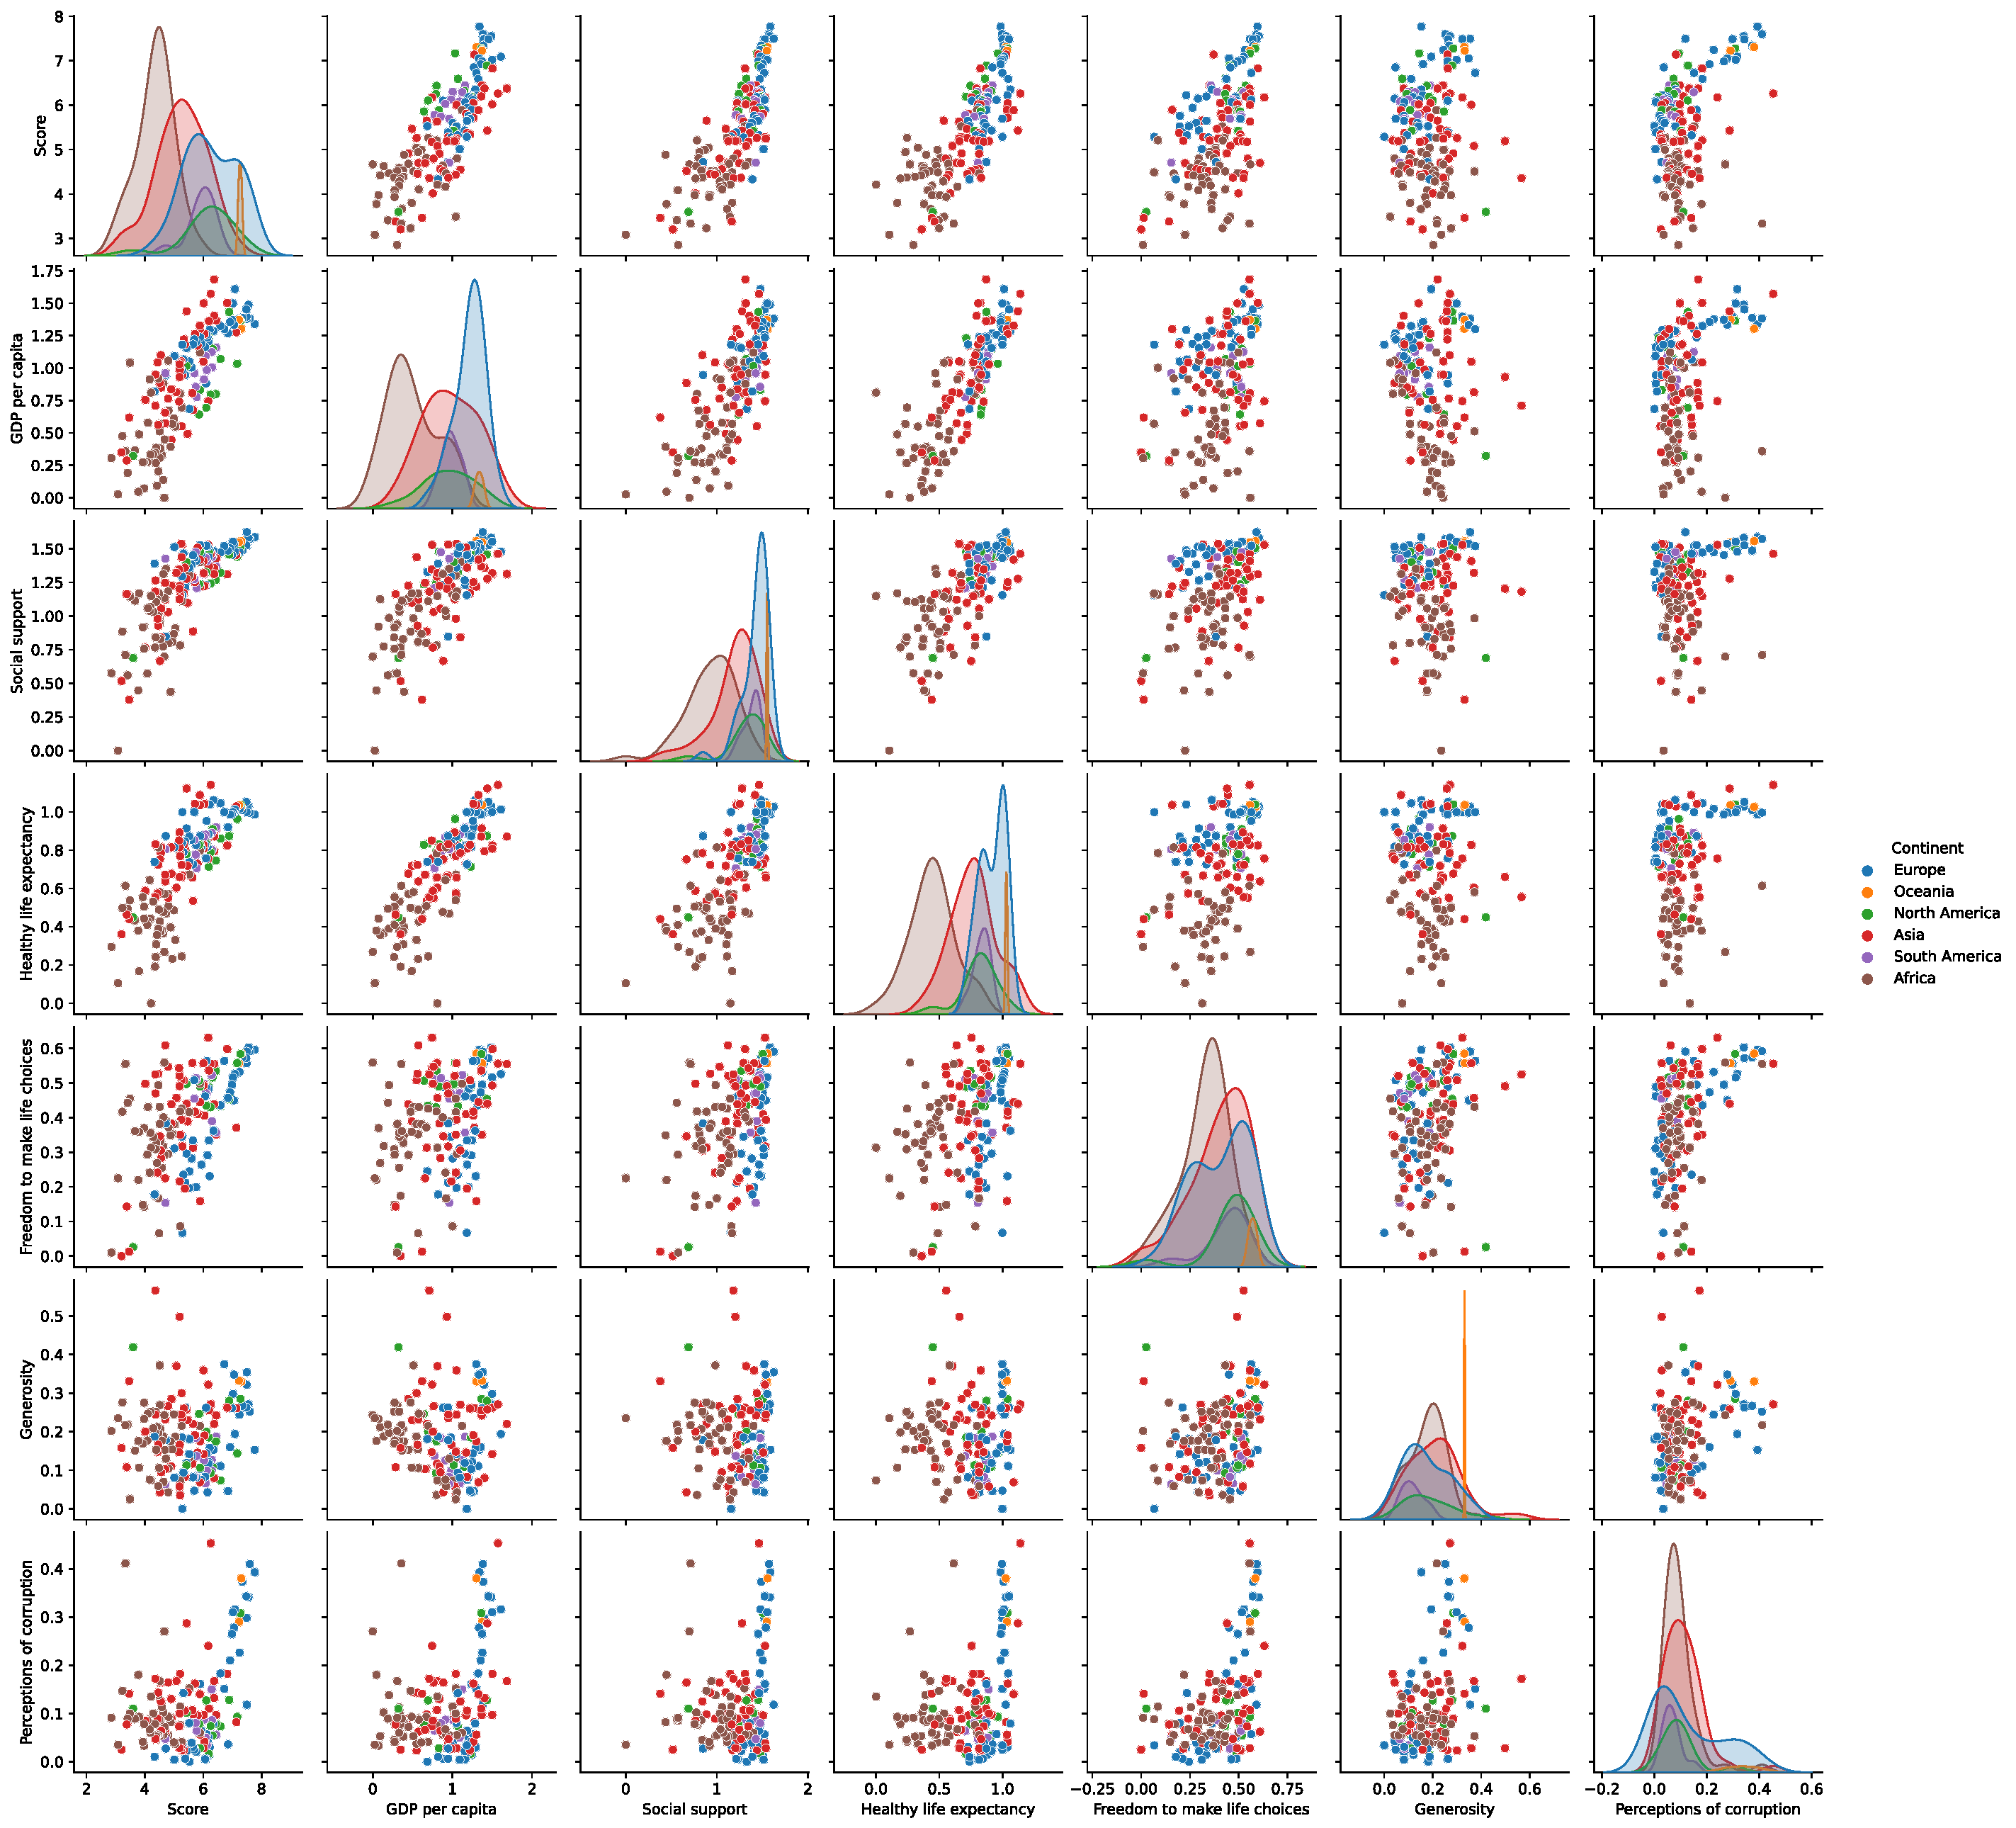
\includegraphics[scale=0.35]{pairplots.pdf}
\centering
\caption{\emph{Relação entre variáveis}}
\label{fig:fig5}
\end{figure}

Analisando a relação do \emph{Score} com as outras variáveis na Figura~\ref{fig:fig5} vemos que existe uma correlação positiva com quase todas as variáveis. Contudo, a generosidade
practicamente não têm influência, e a corrupção apenas se consegue
detectar a presença de correlação em valores elevados. Algumas correlações positivas
esperadas comprovam-se, tal como \emph{PIB per capita} e \emph{Apoio
social}, \emph{PIB per capita} e \emph{esperança média de vida}, e por
último \emph{Apoio social} e \emph{esperança média de vida}. Nota para o
facto de não se conseguir identificar nenhuma correlação
negativa. Antes de passar para a análise do
mapa de correlações, notar que existe uma visível correlação positiva
entre a \emph{percepção de corrupção} e \emph{liberdade}, o que de certa
forma é expectável, tendo em conta que os países no mundo com maior
liberdade são também os que apresentam maior transparência nos seus
processos governamentais.

\begin{figure}[h]
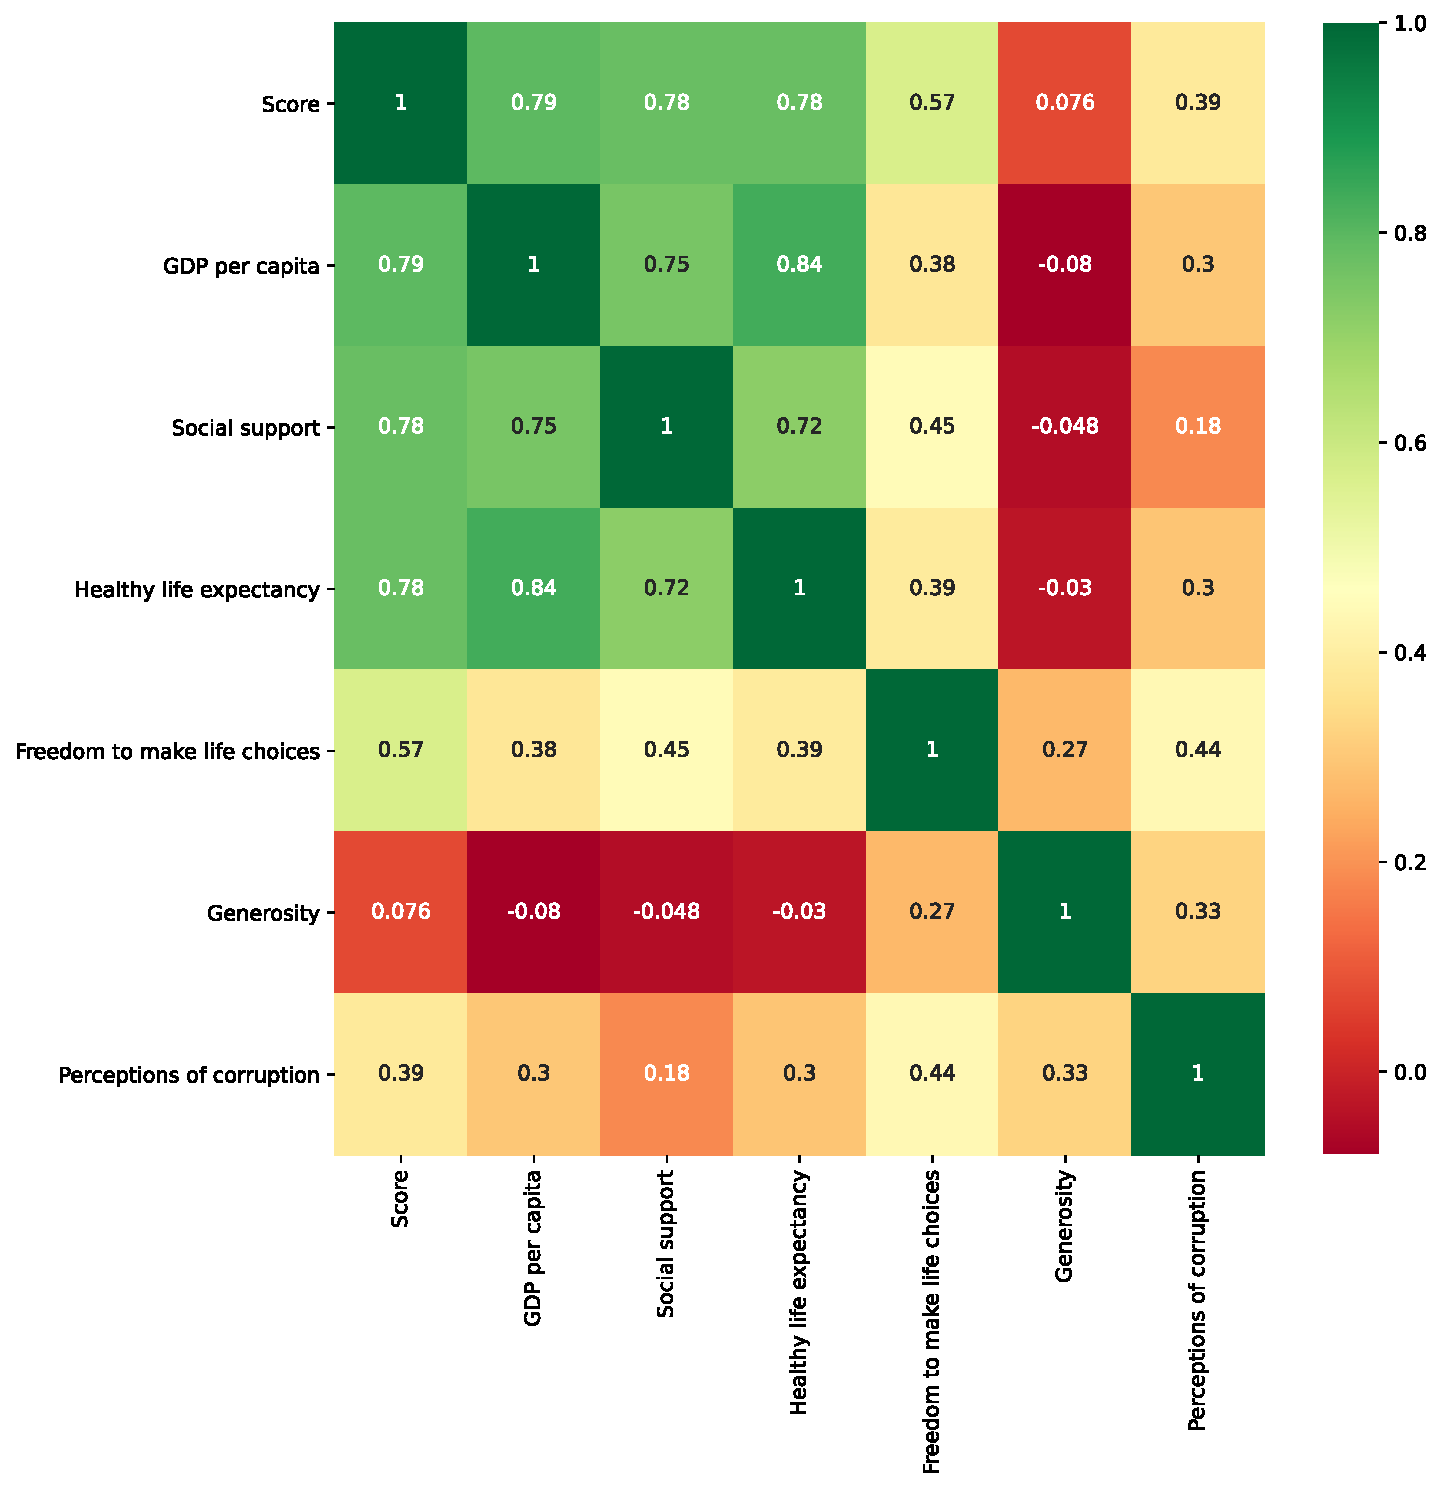
\includegraphics[scale=0.60]{corrmap.pdf}
\centering
\caption{\emph{Mapa de correlações}}
\label{fig:fig6}
\end{figure}

Analisando o mapa de correlações ilustrado na Figura~\ref{fig:fig6} vemos que vai de encontro às conclusões
obtidas anteriormente. Fortes correlações positivas entre as quatro
primeiras variáveis, a muito reduzida presença de correlações negativas
( e com valores muito próximos de zero) e a correlação positiva, embora
não relevante, entre a \emph{percepção de corrupção} e \emph{liberdade}.
% subsection análise_bivariada (end)


% section análise_de_dados (end)


\section{\emph{Factor Analysis}} % (fold)
\label{sec:factor_analisys}

\subsection{Normalização} % (fold)
\label{sub:normalização}

Uma vez que as variáveis têm diferentes escalas, por exemplo o
\emph{Score} varia entre 0 e 10, ao passo que a perceção de corrupção
encontra-se entre 0 e 1 (uma vez que se trata de uma média que avalia as
resposta a uma pergunta com a possibilidade de responder sim (1) ou não
(0)) procedeu-se à normalização dos valores (com remoção da média e
variância unitária) em todas as variáveis com exceção da \emph{Country
or Region}, visto se tratar de uma variável categórica nominal.

% subsection normalização (end)

\subsection{Testes de adequação} % (fold)
\label{sub:testes_de_adequação}

Inicialmente foi aplicado o teste de \emph{Bartlett} sobre os dados
normalizados, sendo a hipótese nula a matriz de correlações trata-se de
uma matriz de identidade, o que indicaria que as variáveis seriam não
correlacionadas e portanto, não adequadas para \emph{factor analysis}
(FA).
Obteve-se um valor de chi-quadrado de aproximadamente 656 e o nível de
significância obtido foi de 0.0 (\(5*10^{-126}\)) indicando a rejeição
da hipótese e, portanto, que os dados são adequados ao tipo de análise
em questão \cite{kaiser}.

Foi, também, realizado o teste
de adequação \emph{Kaiser-Meyer-Olkin's} (KMO), obtendo-se o valor de
aproximadamente 0.84 o que evidencia uma forte adequação à realização de
FA. A Tabela~\ref{tab:tab2} exibe os valores de \emph{Measure of Sampling
Adequacy} (MSA) para as variáveis em análise. Todos as variáveis possuem
um MSA superior a 0.5, tendo sido portanto mantidas para análise \cite{kaiser}.

\begin{table}[h]
\centering
\begin{tabular}{|c|c|c|c|c|c|c|}
\hline
\textit{\textbf{Score}} & \textit{\textbf{GDP}} & \textit{\textbf{\begin{tabular}[c]{@{}c@{}}Social\\ Support\end{tabular}}} & \textit{\textbf{\begin{tabular}[c]{@{}c@{}}Healthy\\ life exp.\end{tabular}}} & \textit{\textbf{Freedom}} & \textit{\textbf{Generosity}} & \textit{\textbf{Corruption}} \\ \hline
0.855 & 0.827 & 0.871 & 0.862 & 0.829 & 0.596 & 0.752 \\ \hline
\end{tabular}
\caption{\emph{Measure of Sampling Analysis}}
\label{tab:tab2}
\end{table}

% subsection testes_de_adequação (end)

\subsection{PCA e Análise} % (fold)
\label{sub:pca_e_análise}

Procedeu-se à aplicação da PCA sobre os dados normalizados, tendo-se obtidos os eigenvalues
apresentados na Tabela~\ref{tab:tab3}:

\begin{table}[h]
\centering
\begin{tabular}{c|c|c|c|}
\cline{2-4}
 & \textbf{Eigenvalue} & \textbf{\begin{tabular}[c]{@{}c@{}}Fracção de Variância\\ Explicada (\%)\end{tabular}} & \textbf{Fracção Acumulada (\%)} \\ \hline
\multicolumn{1}{|c|}{1} & 3.837141 & 54.46 & 54.46 \\ \hline
\multicolumn{1}{|c|}{2} & 1.436346 & 20.39 & 74.85 \\ \hline
\multicolumn{1}{|c|}{3} & 0.616839 & 8.76 & 83.61 \\ \hline
\multicolumn{1}{|c|}{4} & 0.559896 & 7.95 & 91.56 \\ \hline
\multicolumn{1}{|c|}{5} & 0.263794 & 3.74 & 95.30 \\ \hline
\multicolumn{1}{|c|}{6} & 0.173418 & 2.46 & 97.76 \\ \hline
\multicolumn{1}{|c|}{7} & 0.157726 & 2.24 & 100.00 \\ \hline
\end{tabular}
\caption{\emph{Valores dos Eigenvalues}}
\label{tab:tab3}
\end{table}

Na Figura~\ref{fig:fig7} podemos observar a representação gráfica da anterior
tabela:

\begin{figure}[h]
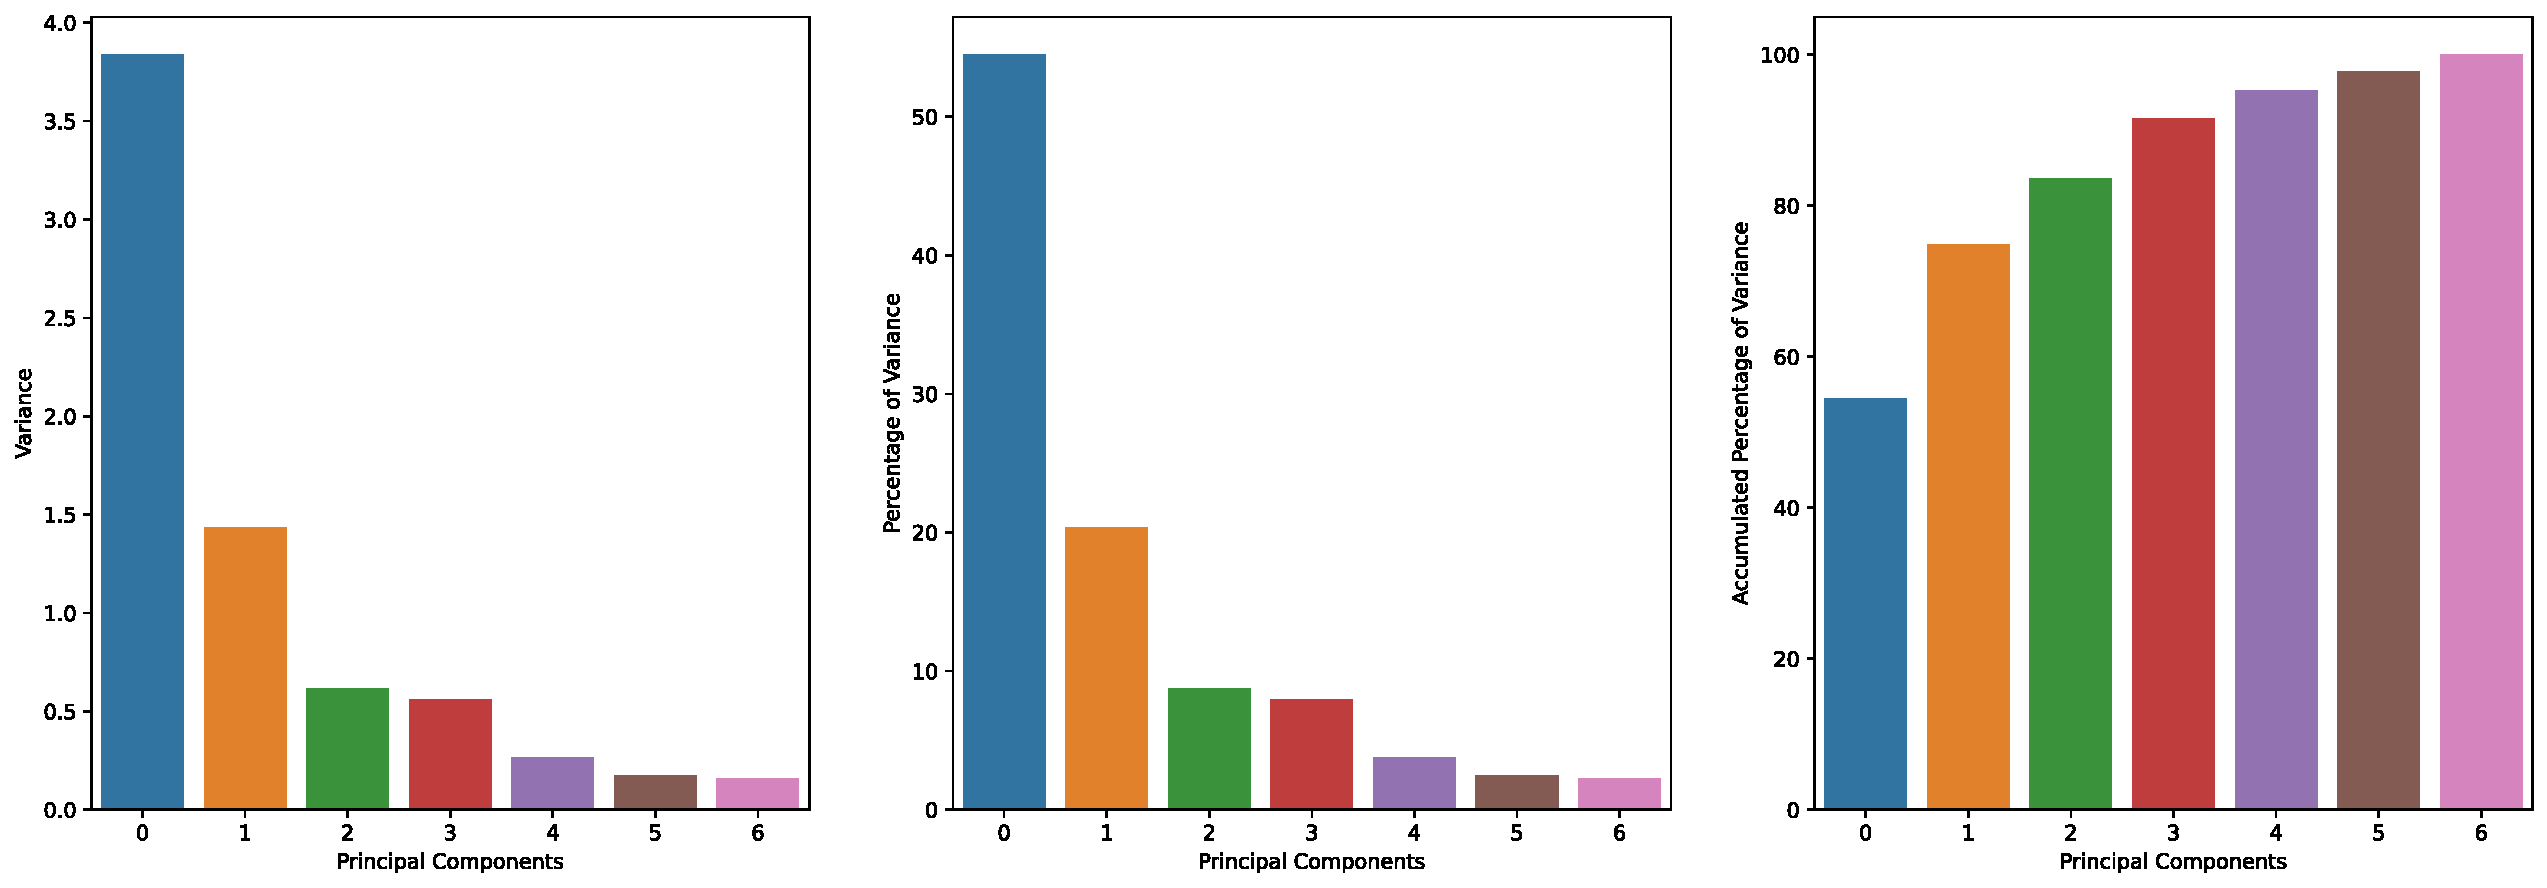
\includegraphics[scale=0.37]{PrincipalComponents.pdf}
\centering
\caption{\emph{Mapa de correlações}}
\label{fig:fig7}
\end{figure}

Verifica-se que a primeira e segundas componentes explicam
aproximadamente 54\% e 20 \% da variância, totalizando 74.85\% da
variância total, sendo que para as componentes seguintes existe uma
queda brusca relativamente a estas. Aplicando o critério de \emph{Kaiser}
(selecionar apenas as componentes a que corresponde um \emph{eigenvalue}
superior a 1) foram selecionadas as primeiras duas componentes (PC1 e
PC2). Na Tabela~\ref{tab:tab4} apresentam-se os \emph{loadings} das primeiras 2 componentes, que representam as
correlações entre as componentes e as variáveis, valores (absolutos)
mais elevados de correlação encontram-se realçados. Estes valores
refletem a importância de cada variável nas componentes.


\begin{table}[h]
\centering
\begin{tabular}{|l|c|c|}
\hline
\textit{\textbf{Features}} & \textbf{PC1} & \textbf{PC2} \\ \hline
\textit{Score} & \cellcolor[HTML]{FFCC67}-0.475861 & -0.028371 \\ \hline
\textit{GDP} & \cellcolor[HTML]{FFCC67}-0.454825 & -0.213377 \\ \hline
\textit{Healthy life exp} & \cellcolor[HTML]{FFCC67}-0.436582 & -0.207148 \\ \hline
\textit{Social support} & \cellcolor[HTML]{FFCC67}-0.450150 & -0.177856 \\ \hline
\textit{Freedom} & -0.332201 & 0.362130 \\ \hline
\textit{Generosity} & -0.048232 & \cellcolor[HTML]{FFCC67}0.693809 \\ \hline
\textit{Corruption} & -0.246511 & \cellcolor[HTML]{FFCC67}0.516346 \\ \hline
\end{tabular}
\caption{\emph{Loadings PC1 e PC2}}
\label{tab:tab4}
\end{table}

Seguidamente, na Figura~\ref{fig:fig8} podemos observar os dados dos \emph{loadings} no círculo de
correlação. Como se pode visualizar a PC1 está mais correlacionada com
as variáveis \emph{Score, GDP, Social support and Healthy life exp.}, ao
passo que a PC2 está mais ligada às 3 restantes
variáveis.

\begin{figure}[h]
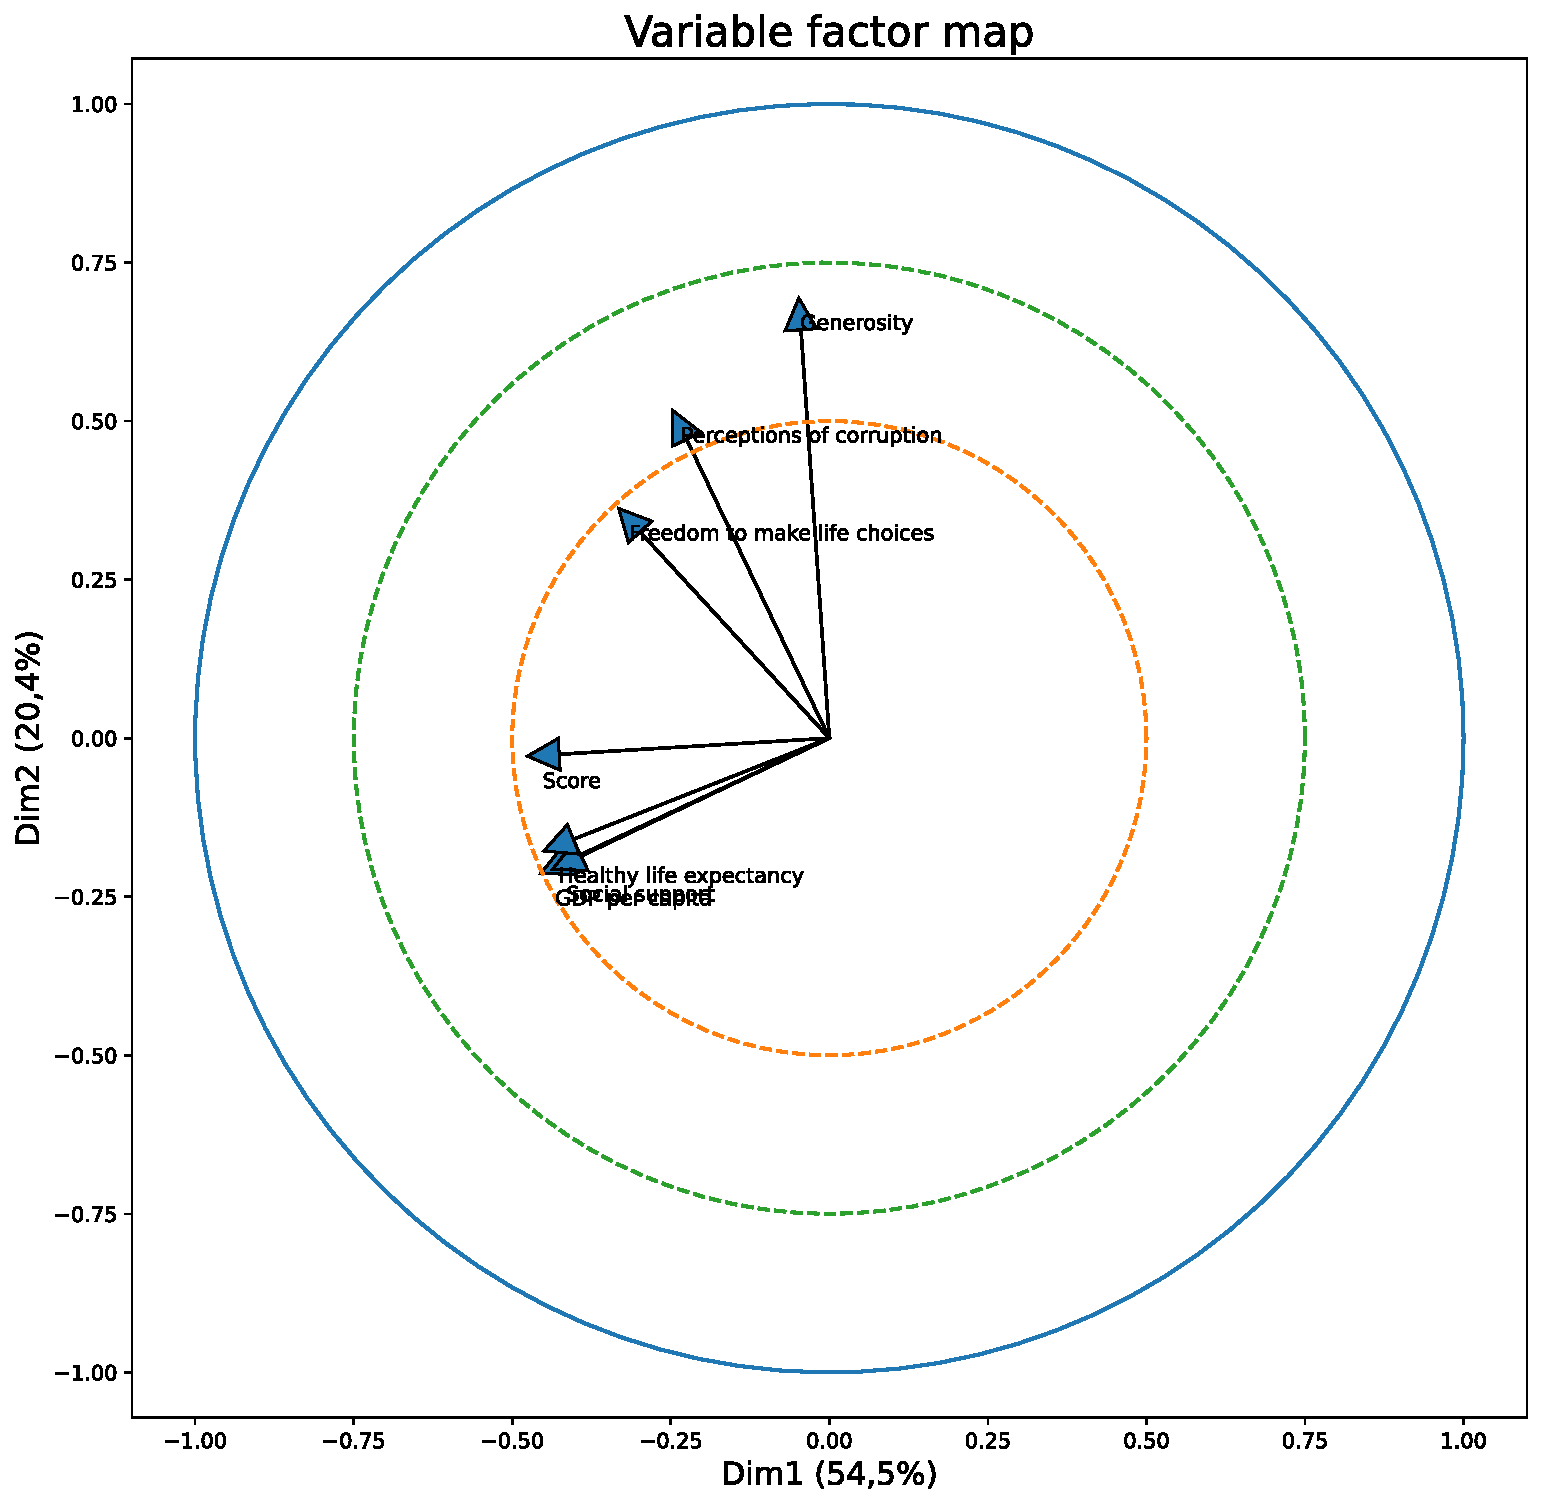
\includegraphics[scale=0.40]{VariableFactorMap1.pdf}
\centering
\caption{\emph{Circulo de correlações}}
\label{fig:fig8}
\end{figure}

Foi aplicada FA com duas
componentes tendo sido utilizada uma rotação (de forma a melhorar a
interpretação) do tipo \emph{varimax} e o método de eixo principal para
realizar a extração, tendo-se obtido as \emph{loadings, communalities} e
variância específica representadas na Tabela~\ref{tab:tab5}:

\begin{table}[h]
\centering
\begin{tabular}{l|c|c|c|c|}
\cline{2-5}
 & \textit{\textbf{Factor 1}} & \textit{\textbf{Factor 2}} & \textit{\textbf{Communalities}} & \textit{\textbf{Variância específica}} \\ \hline
\multicolumn{1}{|l|}{\textit{\textbf{Score}}} & 0.886962 & 0.278875 & 0.864474 & 0.14 \\ \hline
\multicolumn{1}{|l|}{\textit{\textbf{GDP}}} & 0.922187 & 0.056855 & 0.853661 & 0.15 \\ \hline
\multicolumn{1}{|l|}{\textit{\textbf{Healthy life exp.}}} & 0.886130 & 0.051952 & 0.787925 & 0.21 \\ \hline
\multicolumn{1}{|l|}{\textit{\textbf{Social support}}} & 0.899390 & 0.093791 & 0.817701 & 0.18 \\ \hline
\multicolumn{1}{|l|}{\textit{\textbf{Freedom}}} & 0.466562 & 0.624670 & 0.607894 & 0.39 \\ \hline
\multicolumn{1}{|l|}{\textit{\textbf{Generosity}}} & -0.188509 & 0.812598 & 0.695852 & 0.30 \\ \hline
\multicolumn{1}{|l|}{\textit{\textbf{Corruption}}} & 0.247258 & 0.742319 & 0.612174 & 0.39 \\ \hline
\end{tabular}
\caption{\emph{Resultados da Factor Analysis}}
\label{tab:tab5}
\end{table}

Pela análise da tabela podemos concluir que o Factor 1 está fortemente
relacionado com as primeiras 4 variáveis ao passo que o Factor 2
encontra-se mais correlacionado com as restantes variáveis. Em termos de
\emph{communalities} verifica-se que uma fração significativa das
variáveis é explicada pelo factores presentes. Na Figura~\ref{fig:fig9} está
representado o círculo de correlação das \emph{loadings} obtidas.

\begin{figure}[h!]
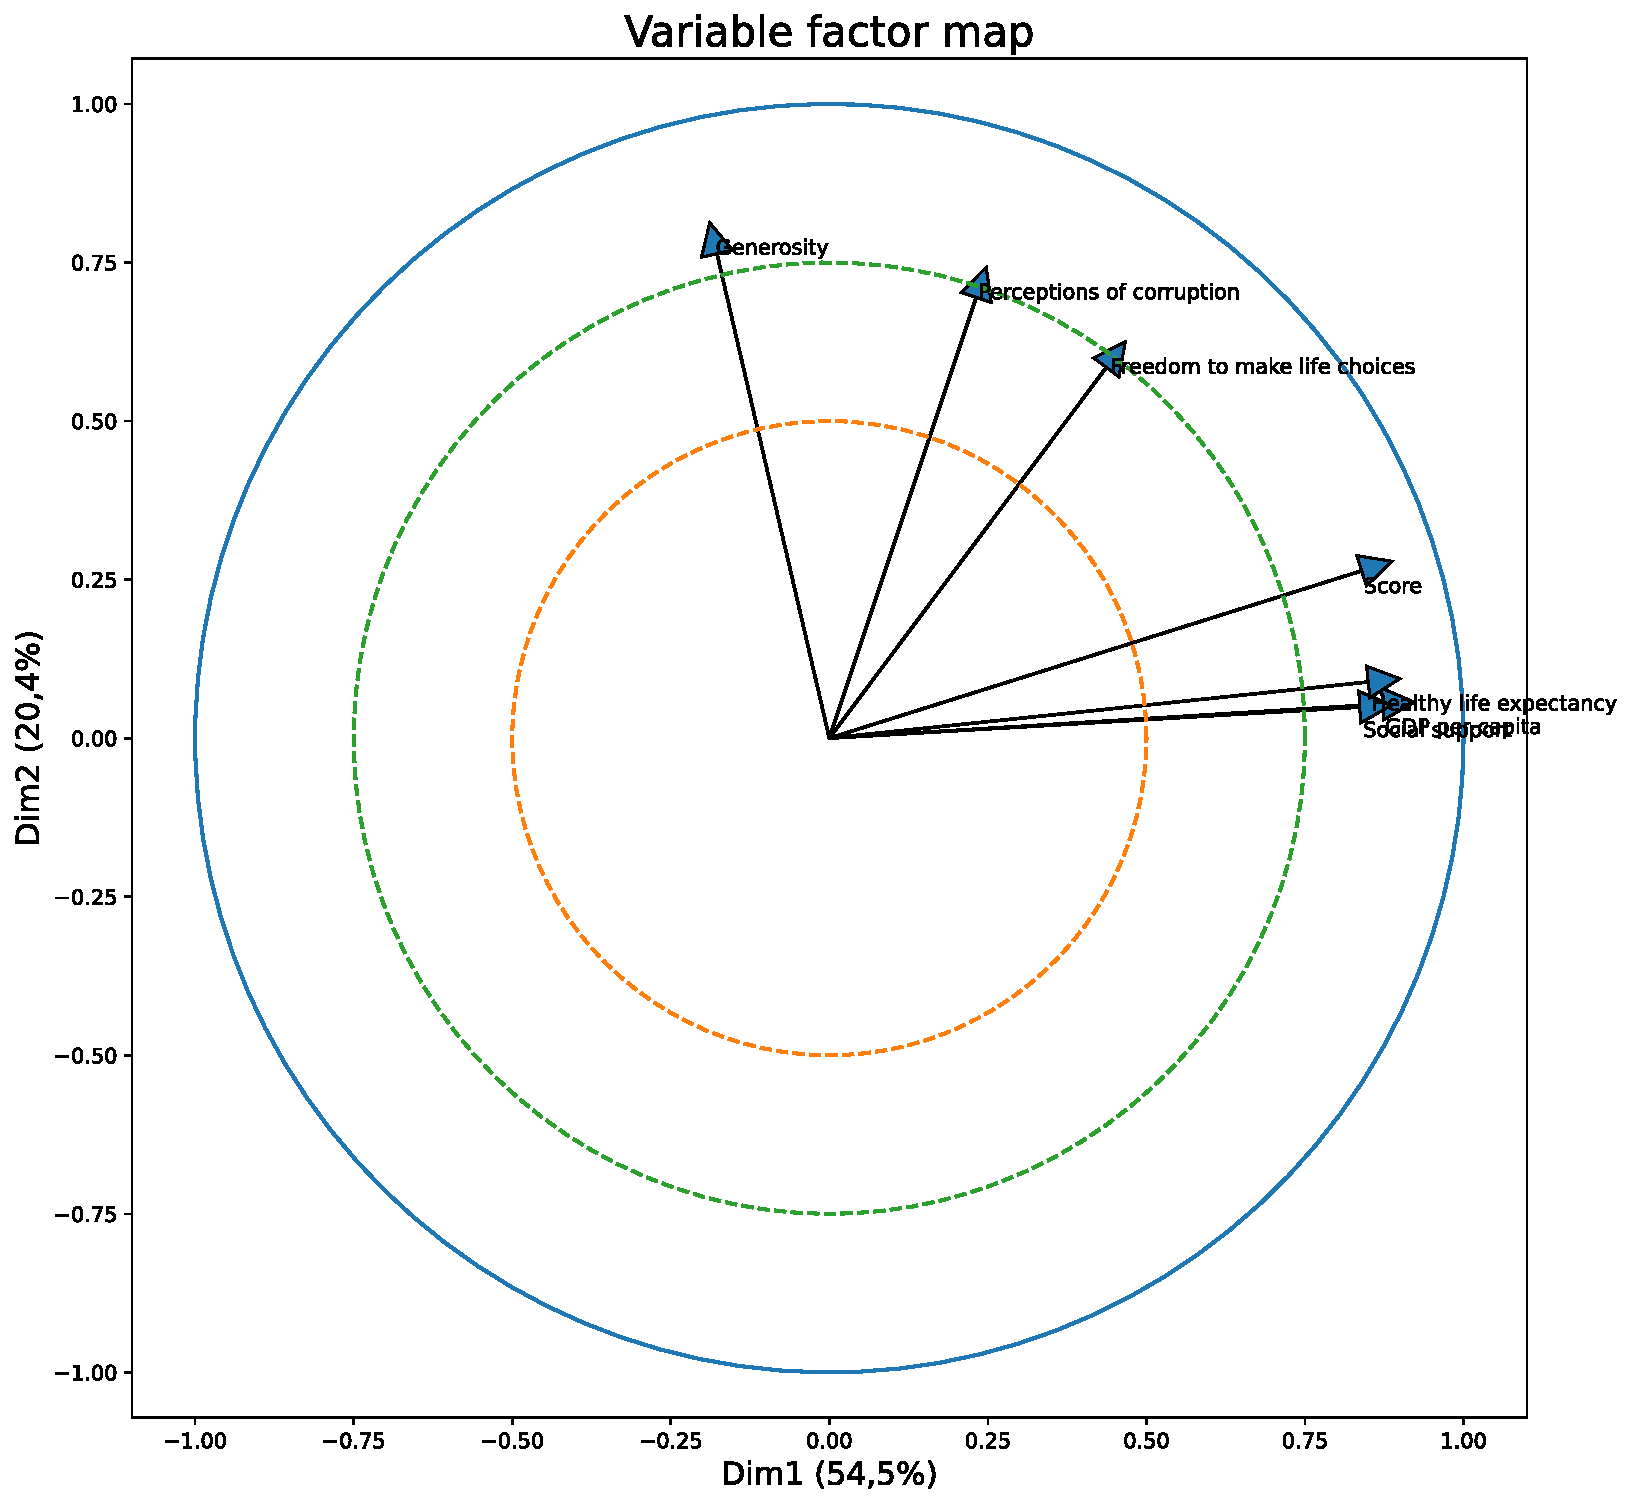
\includegraphics[scale=0.40]{VariableFactorMap2.pdf}
\centering
\caption{\emph{Circulo de correlações}}
\label{fig:fig9}
\end{figure}

Na Figura~\ref{fig:fig10} encontra-se representado o gráfico dos indivíduos
(países) quando a eles é aplicada a transformação imposta pelo modelo
determinado pela FA. Verifica-se que, por exemplo, os países europeus
têm a tendência de estar mais na positiva do eixo das abcissas,
indicando que estes (provavelmente) têm um maior \emph{Score}, esperança
média de vida saudável, GDP e suporte social (uma vez que a correlação
destas variáveis é mais forte com a componente 1. No caso dos países
africanos verifica-se que maioritariamente ocupam as posições do gráfico
mais à esquerda (indicando maus parâmetros em termos de \emph{score},
esperança média de vida saudável, GDP e suporte social).

\begin{figure}[h!]
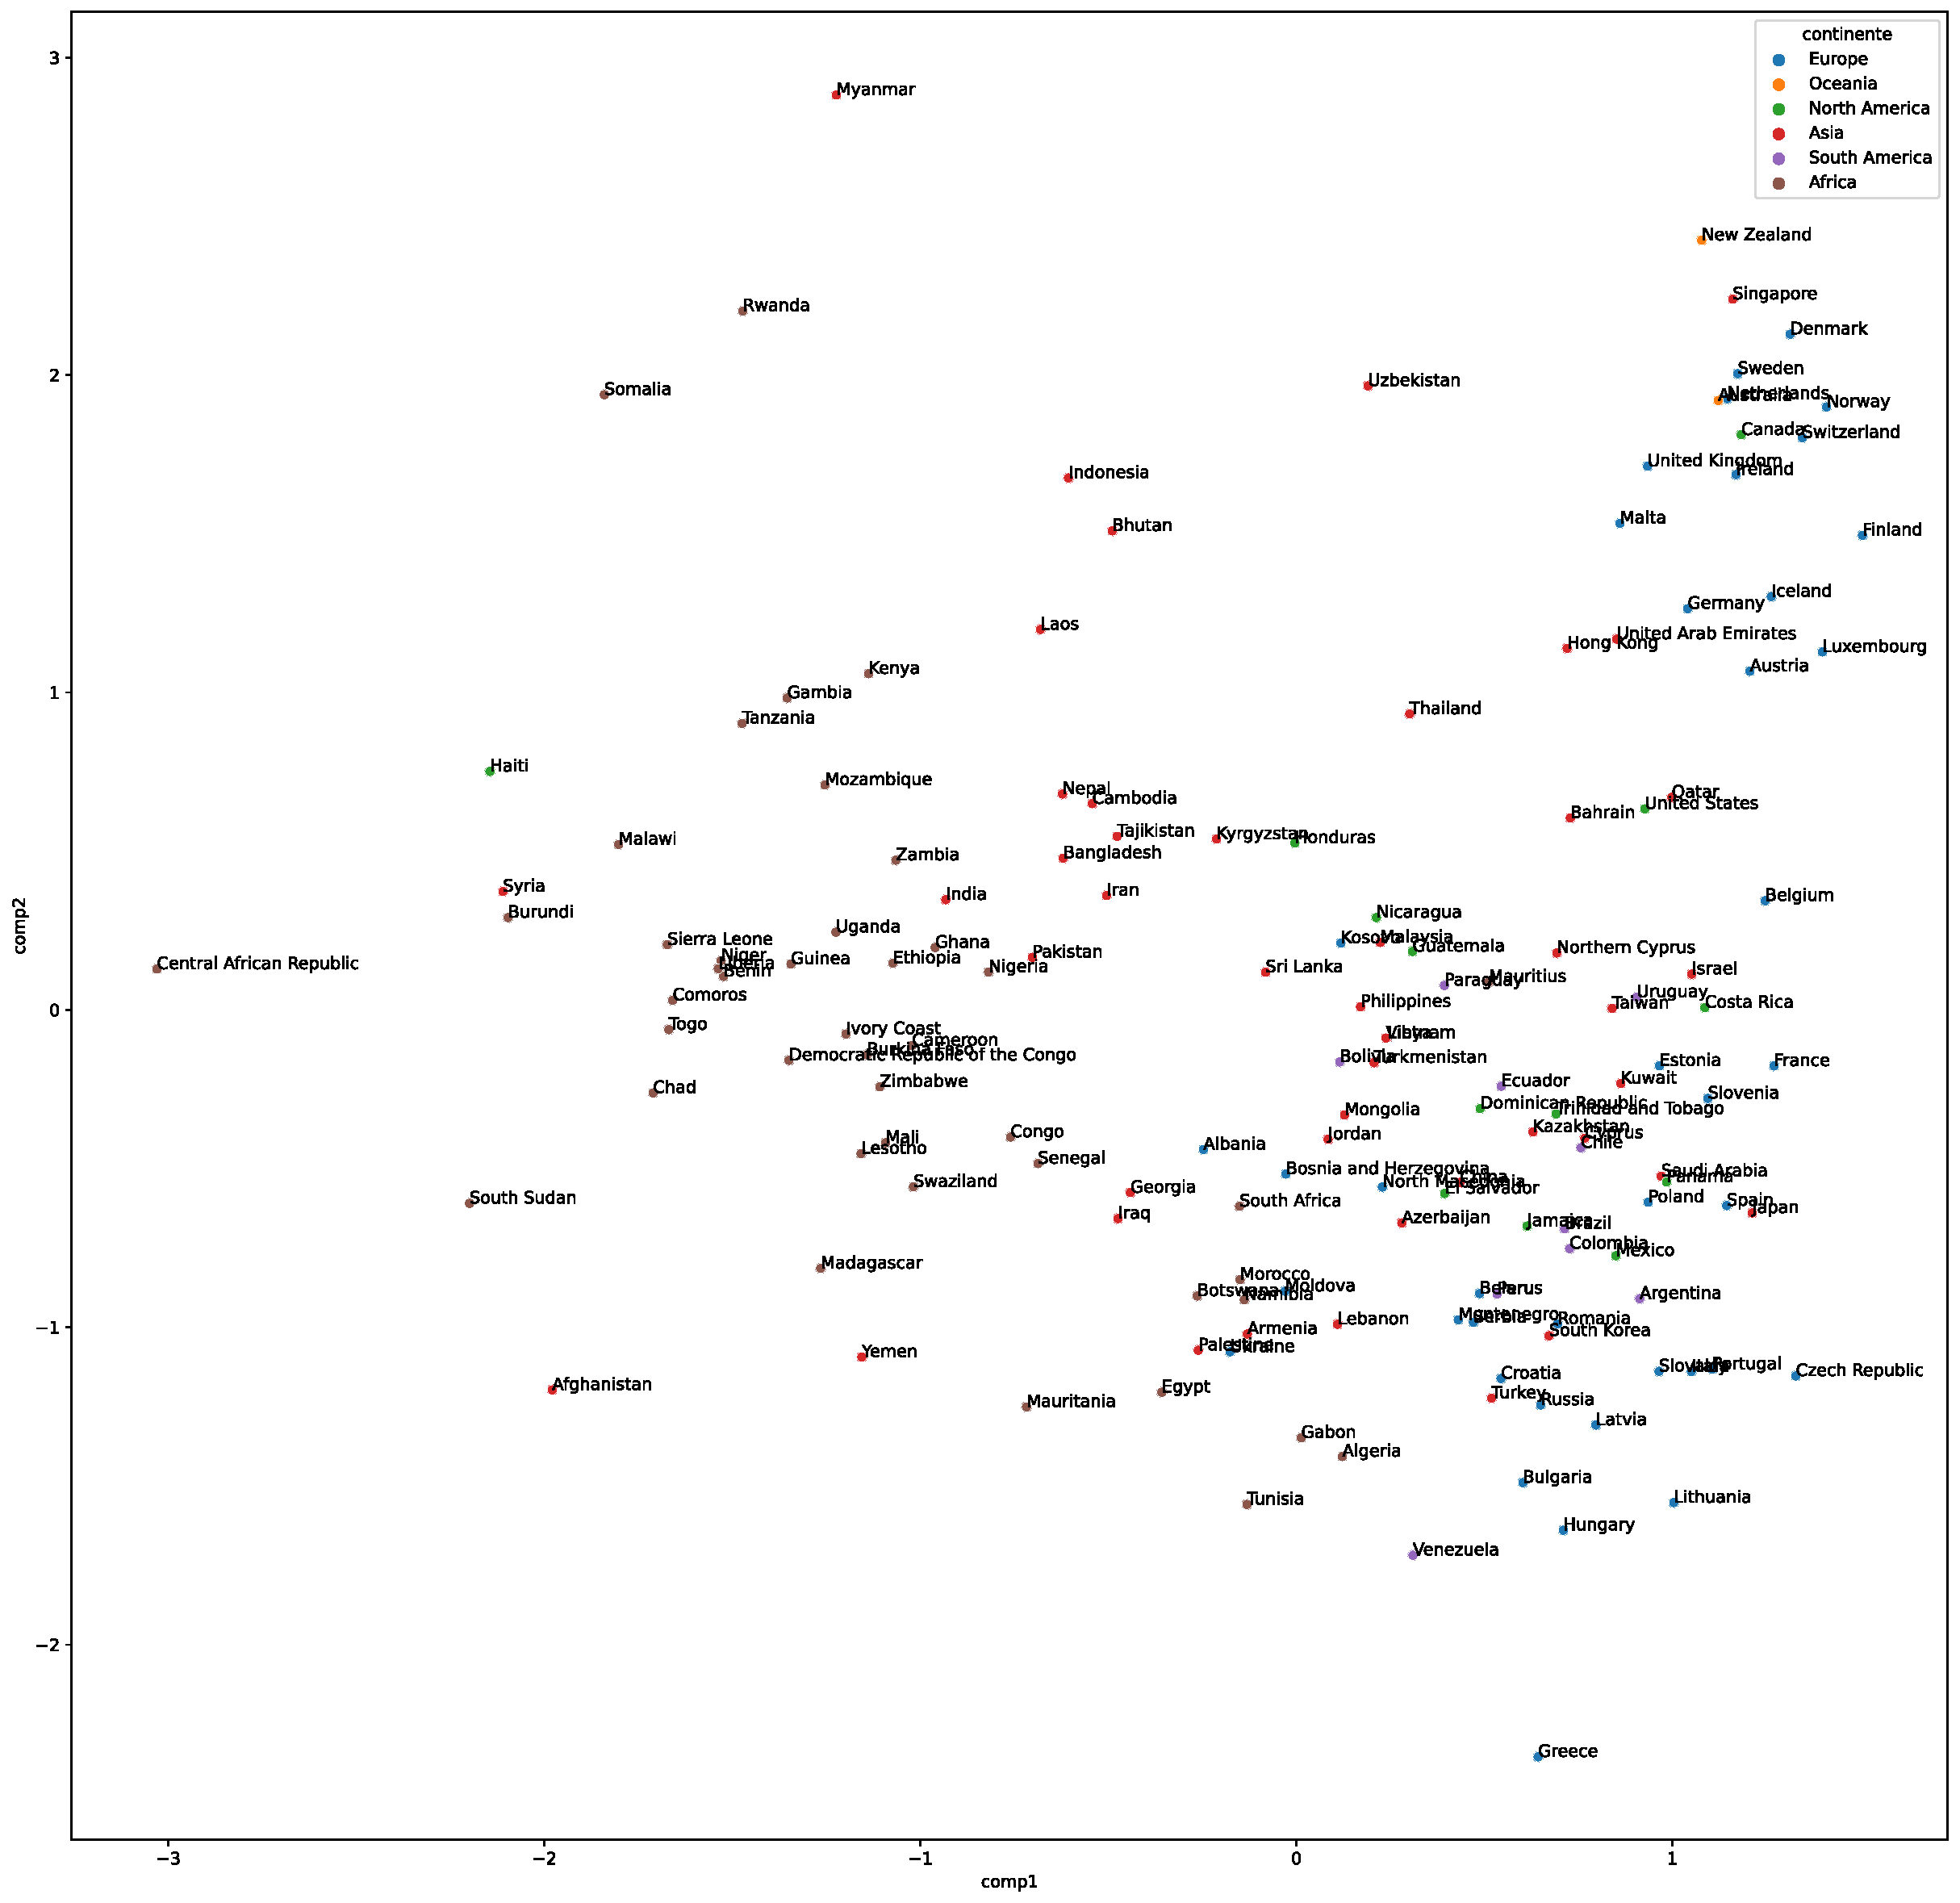
\includegraphics[scale=0.40]{IndividualsMap.pdf}
\centering
\caption{\emph{Representação gráfica dos indivíduos através das transformações aplicadas}}
\label{fig:fig10}
\end{figure}
% subsection pca_e_análise (end)

% section factor_analysis (end)

\section{Conclusão} % (fold)
\label{sec:conclusão}

Com a realização deste trabalho é possível retirar a conclusão de que os
métodos estatísticos abordados são de uma enorme importância para a
escolha de variáveis. Embora o \emph{dataset} escolhido não fosse muito
extenso, foi possível analisar a importância de cada uma das variáveis e
o peso das mesmas.

Encontraram-se algumas
dificuldades, nomeadamente na procura de suporte para alguns métodos na
linguagem \emph{Python}, pois ainda não é tão abrangente neste capítulo
como o \emph{R}.

Após realização de teste de
adequação verificou-se que FA é um método apropriado aos dados em
questão. Constatou-se, através desta análise, que é possível reduzir o
conjunto de dados apresentado, com sete variáveis numéricas, a apenas 2
fatores mantendo quase 75\% da variância total representada.
% section conclusão (end)

\printbibliography


\end{document}